\documentclass[10pt]{article}
\usepackage[a4paper,margin=20mm]{geometry}
\usepackage{mathptmx}
\usepackage[T1]{fontenc}
\usepackage{amsmath}
\usepackage{graphicx}
\usepackage{booktabs}
\usepackage{tabularx}
\usepackage{xcolor}
\usepackage[hidelinks]{hyperref}
\usepackage{cleveref}
\usepackage{caption}
\usepackage{subcaption}
\captionsetup{font=small,labelfont=bf}
\usepackage{enumitem}
\setlist{nosep,leftmargin=*}
\usepackage{float}
\graphicspath{{../figures/}{../figures/maps/}}

\title{\textbf{robot04 Autonomous Mapping: Experiments of 20 October 2026}\\[2pt]
\large Hector SLAM + Nav2 + frontier explorer on the Raspberry~Pi~5}
\author{Marthens Hakizimana and Amir Taghavipour\\
\small Motion and Power Electronics Control (MPEC) Lab, Simon Fraser University\\
\small BCIT Centre for Welding Technologies and Metallurgy Research}
\date{\small Experiment log, 20 October 2026}

\begin{document}
\maketitle

\begin{abstract}
\noindent
On 20 October 2026, robot04 (Hiwonder MentorPi~T1, Raspberry~Pi~5, MS200 lidar) ran
\textbf{18 autonomous exploration runs} between 09:32 and 12:57, driving \textbf{153\,m} in
\textbf{32.5\,min} of explorer time. Hector SLAM, Nav2 and the frontier explorer ran on the robot;
the PC mapper app watched, and \textbf{8 maps} were saved from it. No code changed during the day: the runs
differ in where they ran and how they ended. In a large open area (morning) 82\,\% of Nav2 goals
were aborted and no run got back to its start. Four runs at 10:53 ended within 4\,s on the explorer's
low-battery rule. In a small walled enclosure (afternoon) 7 of 9 runs explored until no frontier was left
and drove home; the last six runs had \textbf{no failed goal} (39 sent). The new mapping timer in the app was
used on the last two runs and agrees with the explorer's own clock to within 12\,s.
\end{abstract}

\section{Setup}
\begin{itemize}
\item \textbf{Robot:} robot04, Raspberry~Pi~5, tracked base, Oradar MS200 360\textdegree{} lidar (10\,Hz).
\item \textbf{On the robot} (\texttt{systemctl --user start robot-explore}): Hector SLAM (0.05\,m cells),
Nav2 (NavFn, Regulated Pure Pursuit at 0.10\,m/s), the frontier explorer
(robot radius 0.15\,m, minimum frontier 0.30\,m, size weight 0.5, replan every 3\,s,
no-progress timeout 30\,s, battery limit 7.0\,V). The parameters were the same in every run
(they are recorded in each log's \texttt{begin} event).
\item \textbf{On the PC:} the robot04 mapper app shows the map, path, plan and frontiers; it saves the
robot's \texttt{/map} as map\_server \texttt{pgm}/\texttt{yaml} plus a JSON note.
\item \textbf{Data} (all in \texttt{experiments/2026-10-20/data}): 18 explorer logs
(\texttt{robot\_logs/*.jsonl}, one event per goal plus a sample every few seconds), 17 maps the
explorer saved on the robot (\texttt{robot\_maps}) and the 8 maps saved from the PC (\texttt{pc\_maps}).
\end{itemize}
A run starts when \textbf{Explore} is pressed and ends when the explorer reports \emph{done} (no frontier left
and back at the start, or a stop condition) or the operator stops it. The duration below is the time
from \emph{start} to that event; the distance is the explorer's sum of SLAM pose steps.
Mapped area is the number of known cells (free or occupied) times 0.05$^2$\,m$^2$; it includes
everything the lidar saw, also beyond walls the robot could not pass.

\section{Runs}
The 18 runs fall into five sessions (\cref{tab:sessions}, \cref{fig:overview}).

\begin{table}[H]
\centering\small
\caption{Sessions. Failed goals: Nav2 aborted the goal or it timed out.}
\label{tab:sessions}
\begin{tabular}{lllrrrrrl}
\toprule
& Time & Conditions & Runs & Home & Failed / sent & Fail & Driven (m) & Completed runs (mean) \\
\midrule
\csname @@input\endcsname sessions_table 
\bottomrule
\end{tabular}
\end{table}

\begin{figure}[H]
\centering
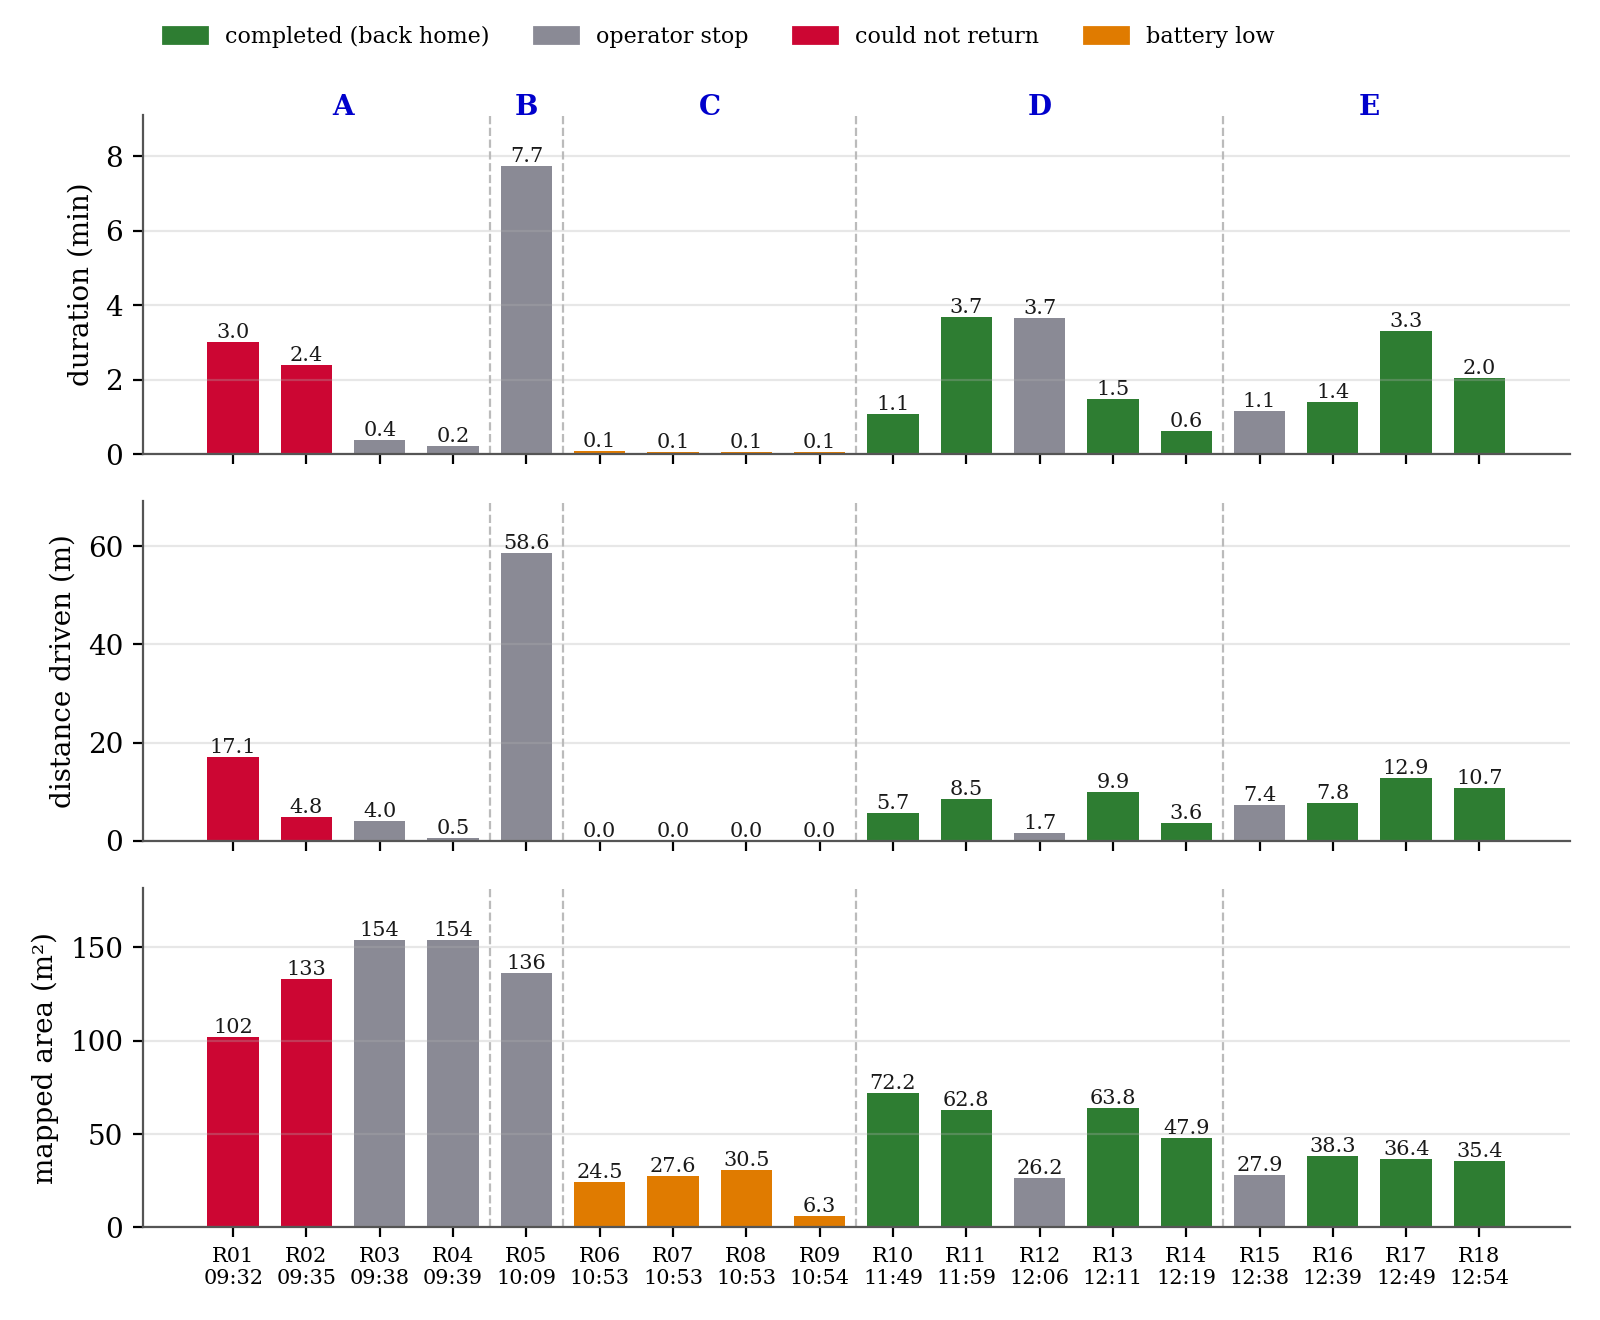
\includegraphics[width=0.92\linewidth]{runs_overview}
\caption{Every run: duration, distance driven and mapped area, coloured by how it ended.
Sessions A--E are separated by dashed lines. In sessions A and C the SLAM map was not reset between
runs, so their mapped area is cumulative.}
\label{fig:overview}
\end{figure}

\begin{table}[H]
\centering\small
\caption{All runs. Reached: frontier goals Nav2 reached; seen: frontiers that disappeared while driving
to them (the lidar saw them first); failed: Nav2 aborted or timed out.}
\label{tab:runs}
\begin{tabular}{lllrrrrrrrl}
\toprule
Run & S. & Start & Time (s) & Dist. (m) & Area (m$^2$) & Sent & Reached & Seen & Failed & End \\
\midrule
\csname @@input\endcsname runs_table 
\bottomrule
\end{tabular}
\end{table}

\subsection*{A, 09:32--09:41: large open area, goals aborted}
The first two runs mapped 100--130\,m$^2$ of a long area (\cref{fig:mapA}), but Nav2 aborted
62 of 74 goals (status 6) and neither run could drive back to its start. Failed goals cluster at the far
edge of the map and beyond walls seen through gaps; the explorer blacklisted each and sent the next,
41 goals in 3 minutes in R01. R03 was stopped by the operator; R04's log ends after 12\,s.
Frontier search took 80--150\,ms per goal on this map (20--70\,ms on the small afternoon maps).
\textit{Not yet known:} why Nav2 aborted so many goals here. Candidates to check are narrow passages under
the 0.45\,m wall clearance of the global costmap, and goals in cells that are free in Hector's map but
inside the inflated costmap.

\subsection*{B, 10:09: one long run}
R05 is the longest run of the day: 7.7\,min, 58.6\,m driven, 136.5\,m$^2$ mapped, 9 goals reached
and 2 failed (\cref{fig:mapB}). It drove along a corridor about 15\,m long and into the branch at its far end;
the operator stopped it before it finished. Map \texttt{lab\_2026-10-20\_1008} was saved from this run.

\subsection*{C, 10:53--10:55: battery low}
Four runs ended within 4\,s of \emph{start}: the explorer cancelled its first goal with
``battery low'' and returned home. The voltage samples in these logs are 7.02--7.06\,V, just above the
7.0\,V limit, but the check uses the instantaneous voltage, which dips under load when the motors start
(\cref{fig:battery}). R05 had ended at 7.07\,V. By 11:49 the battery read 8.18\,V again.

\subsection*{D, 11:49--12:21: small enclosure}
From here on the robot ran inside a small walled enclosure, about 2.5\,m across, whose layout changed between
runs (\cref{fig:mapsDE}). The lidar sees out of the enclosure into the room, so 26--72\,m$^2$ were mapped
while the robot drove 1.7--9.9\,m. Four of five runs finished (no frontier left, back home);
10 of 34 goals failed, outside the enclosure or against its walls, where the robot cannot drive. R12 was stopped
after 3.7\,min with 1.7\,m driven and 5 failed goals.

\subsection*{E, 12:38--12:57: repeat runs, no failures}
Three of four runs finished; R15 was stopped by the operator after 1.1\,min. No goal failed in this
session (31 sent), nor in R13 and R14 before it. R17 reached all 8 of its goals. The completed runs took 1.4--3.3\,min, drove 7.8--12.9\,m
(mean speed 0.08\,m/s, against a 0.10\,m/s cruise speed) and needed 5--14\,s to drive home after the last frontier.

\section{Mapping time}
\Cref{fig:area} shows how the mapped area grew in the completed runs. Each starts steeply (each goal opens
a new view for a 360\textdegree{} lidar) and then levels off while the robot visits the remaining corners.
In R11 the area stayed at 45--47\,m$^2$ for more than 2\,min before the last goals opened another 16\,m$^2$.

The mapper app's new timer (it runs while SLAM poses arrive) was used for the last two maps
(\cref{tab:maps}): 211\,s against the explorer's 199\,s for R17, and 130\,s against 123\,s for R18.
The timer reads longer because it also counts the seconds between starting SLAM and pressing
\emph{Explore}, and between the end of the run and saving the map. Use the explorer time for the time to map an area, and the app timer for the whole session.

\begin{figure}[H]
\centering
\begin{minipage}[t]{0.56\linewidth}
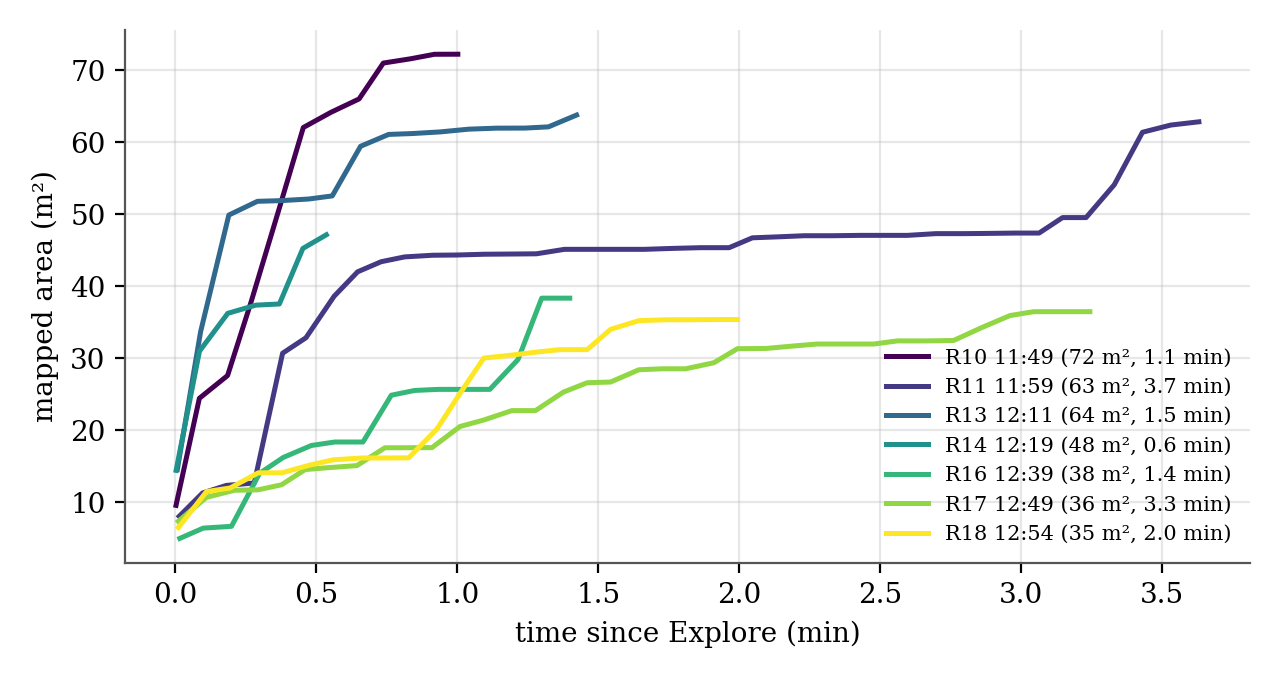
\includegraphics[width=\linewidth]{area_vs_time}
\caption{Mapped area against time since \emph{Explore}, completed runs.}
\label{fig:area}
\end{minipage}\hfill
\begin{minipage}[t]{0.42\linewidth}
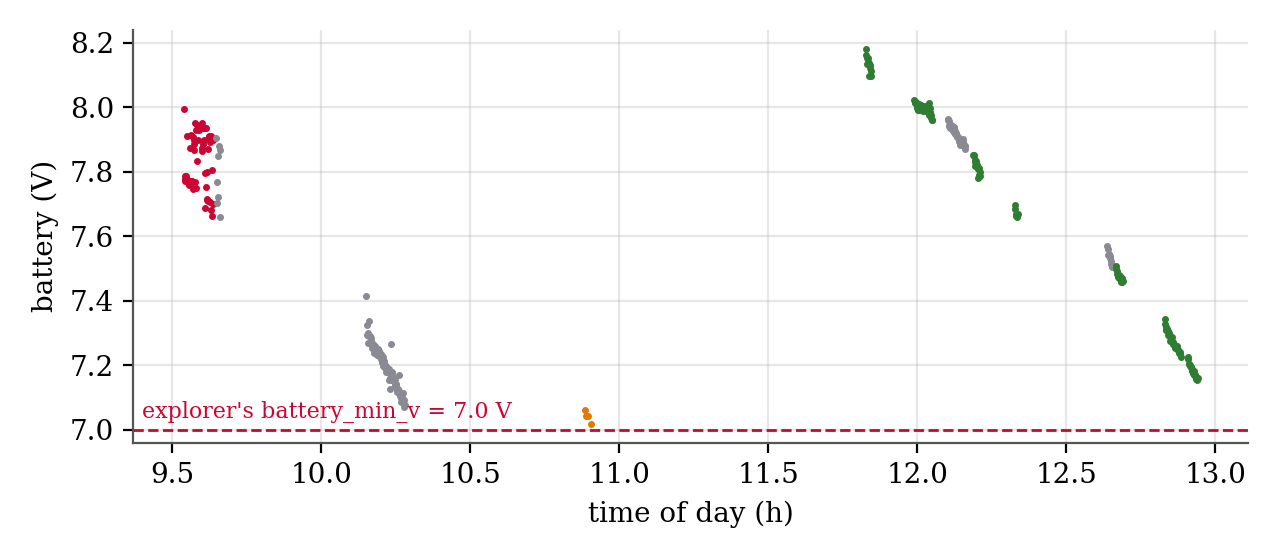
\includegraphics[width=\linewidth]{battery}
\caption{Battery voltage in every log sample, coloured by run outcome (orange: battery low).}
\label{fig:battery}
\end{minipage}
\end{figure}

\begin{figure}[H]
\centering
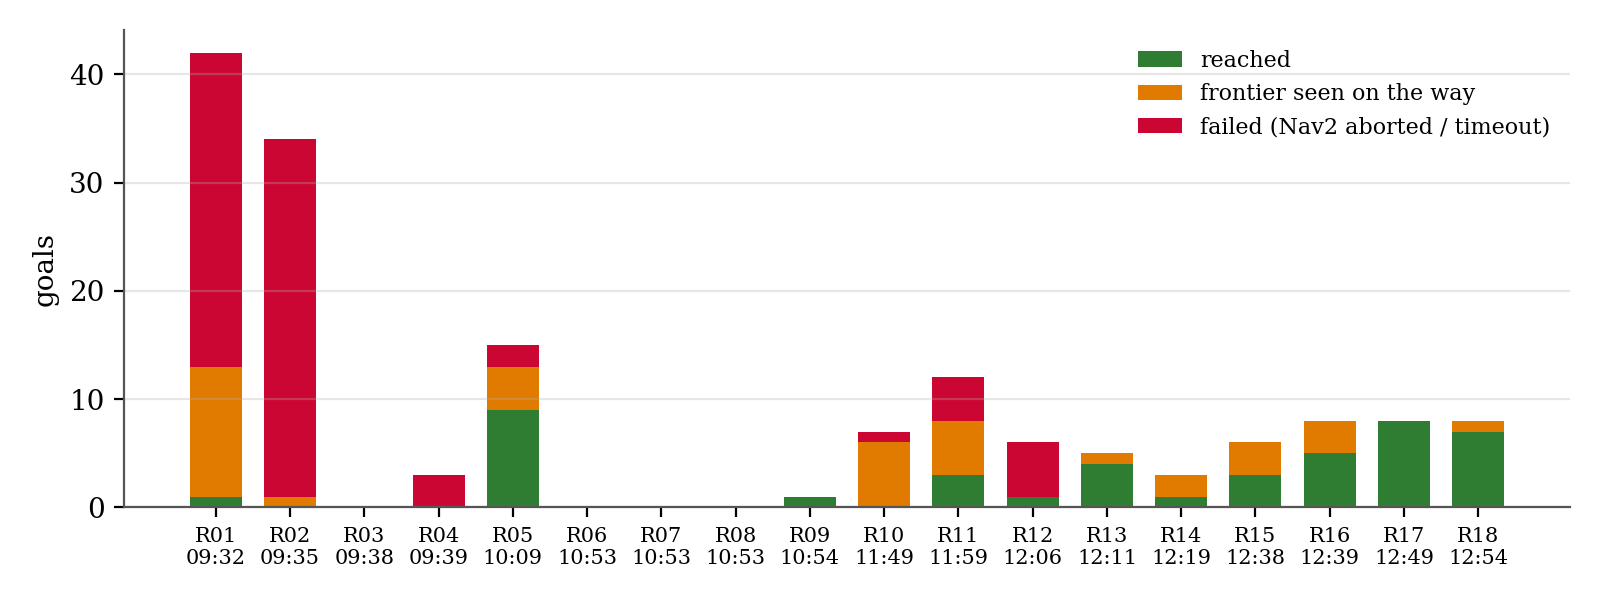
\includegraphics[width=0.85\linewidth]{goal_outcomes}
\caption{Goal outcomes per run.}
\label{fig:goals}
\end{figure}

\section{Saved maps}
\begin{table}[H]
\centering\small
\caption{Maps saved from the PC app (\texttt{lab\_2026-10-20\_*}). Known area = free + occupied.
Timer: app timer / explorer time (s).}
\label{tab:maps}
\begin{tabular}{lllrrrrrr}
\toprule
Map & Saved & Run & Extent (m) & Known (m$^2$) & Free & Occupied & Path (m) & Timer (s) \\
\midrule
\csname @@input\endcsname maps_table 
\bottomrule
\end{tabular}
\end{table}

Every map is plotted with metric axes (x, y in the SLAM map frame, origin at the robot's start),
the robot's path from the explorer's log and the goals. The figures are in \texttt{figures/maps/}.

\begin{figure}[H]
\centering
\begin{subfigure}[t]{0.49\linewidth}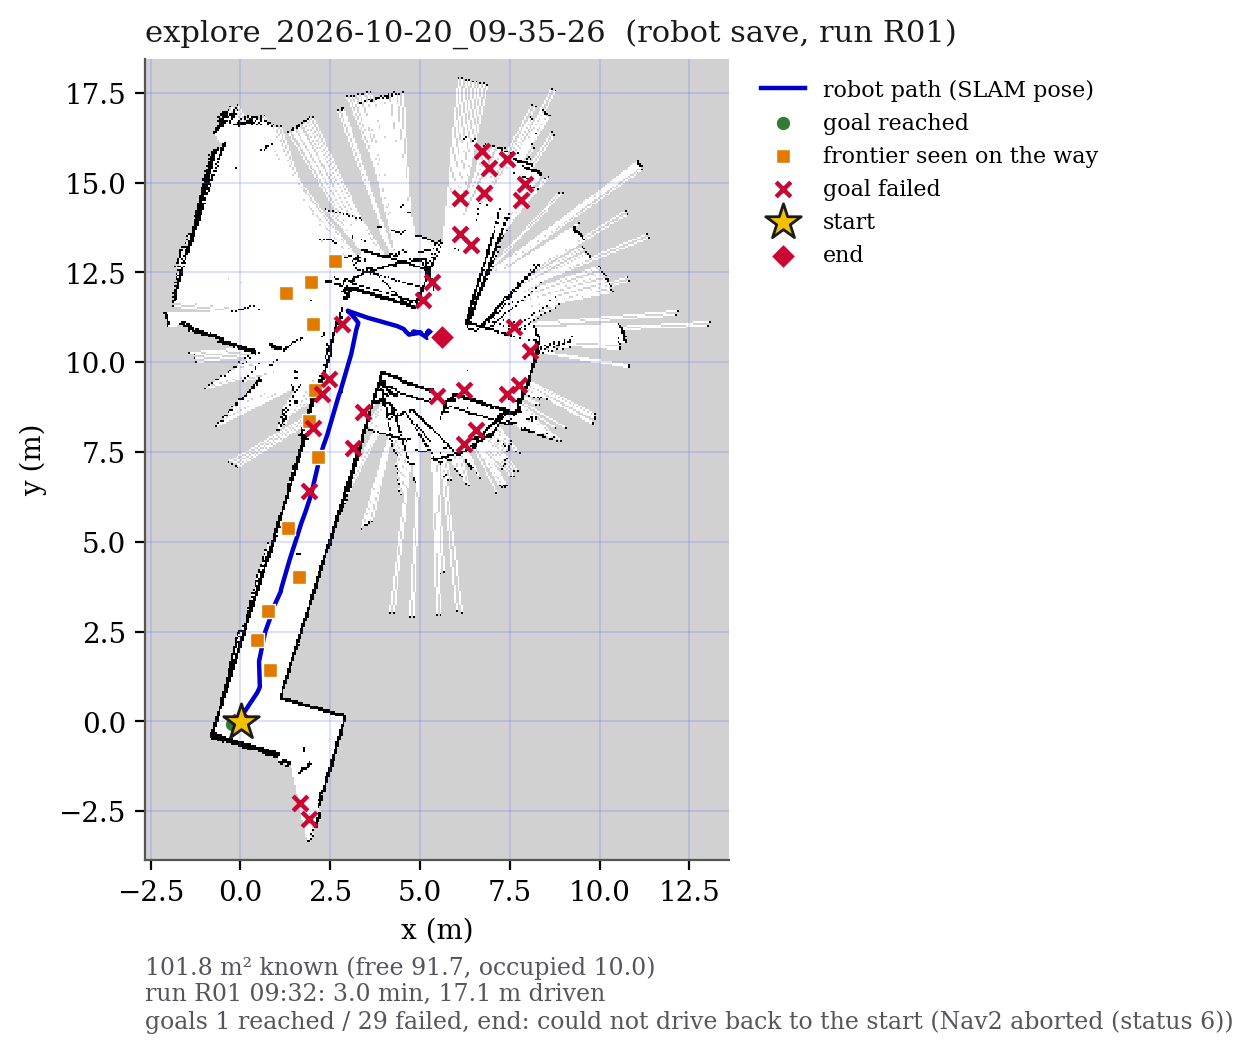
\includegraphics[width=\linewidth]{explore_2026-10-20_09-35-26}
\caption{R01 (session A), robot's own save.}\label{fig:mapA}\end{subfigure}\hfill
\begin{subfigure}[t]{0.49\linewidth}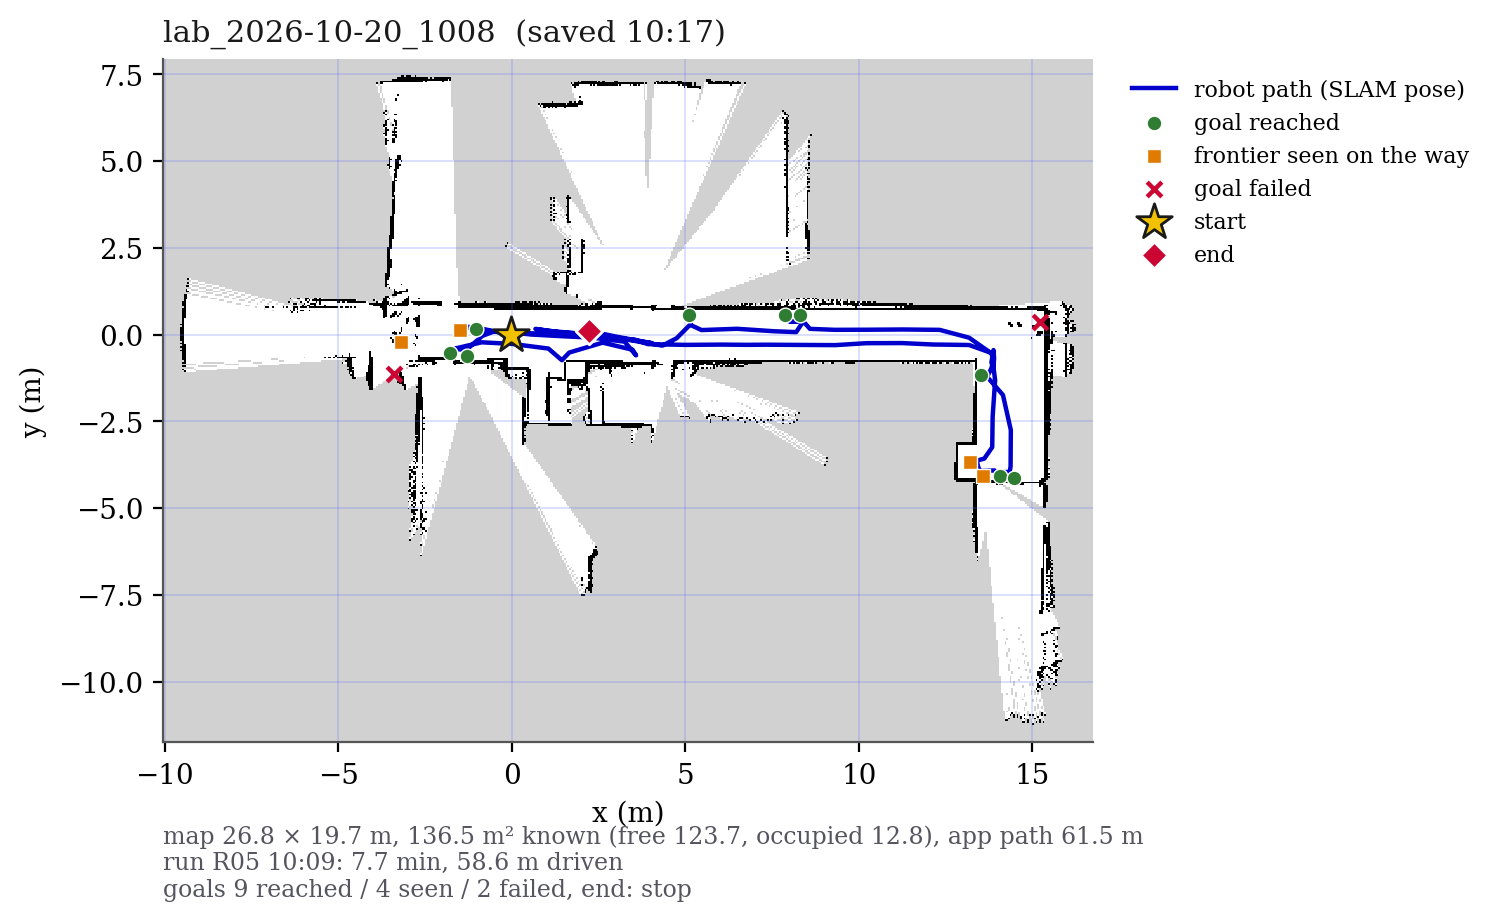
\includegraphics[width=\linewidth]{lab_2026-10-20_1008}
\caption{R05 (session B).}\label{fig:mapB}\end{subfigure}
\caption{Large-area runs.}
\end{figure}

\begin{figure}[H]
\centering
\begin{subfigure}[t]{0.49\linewidth}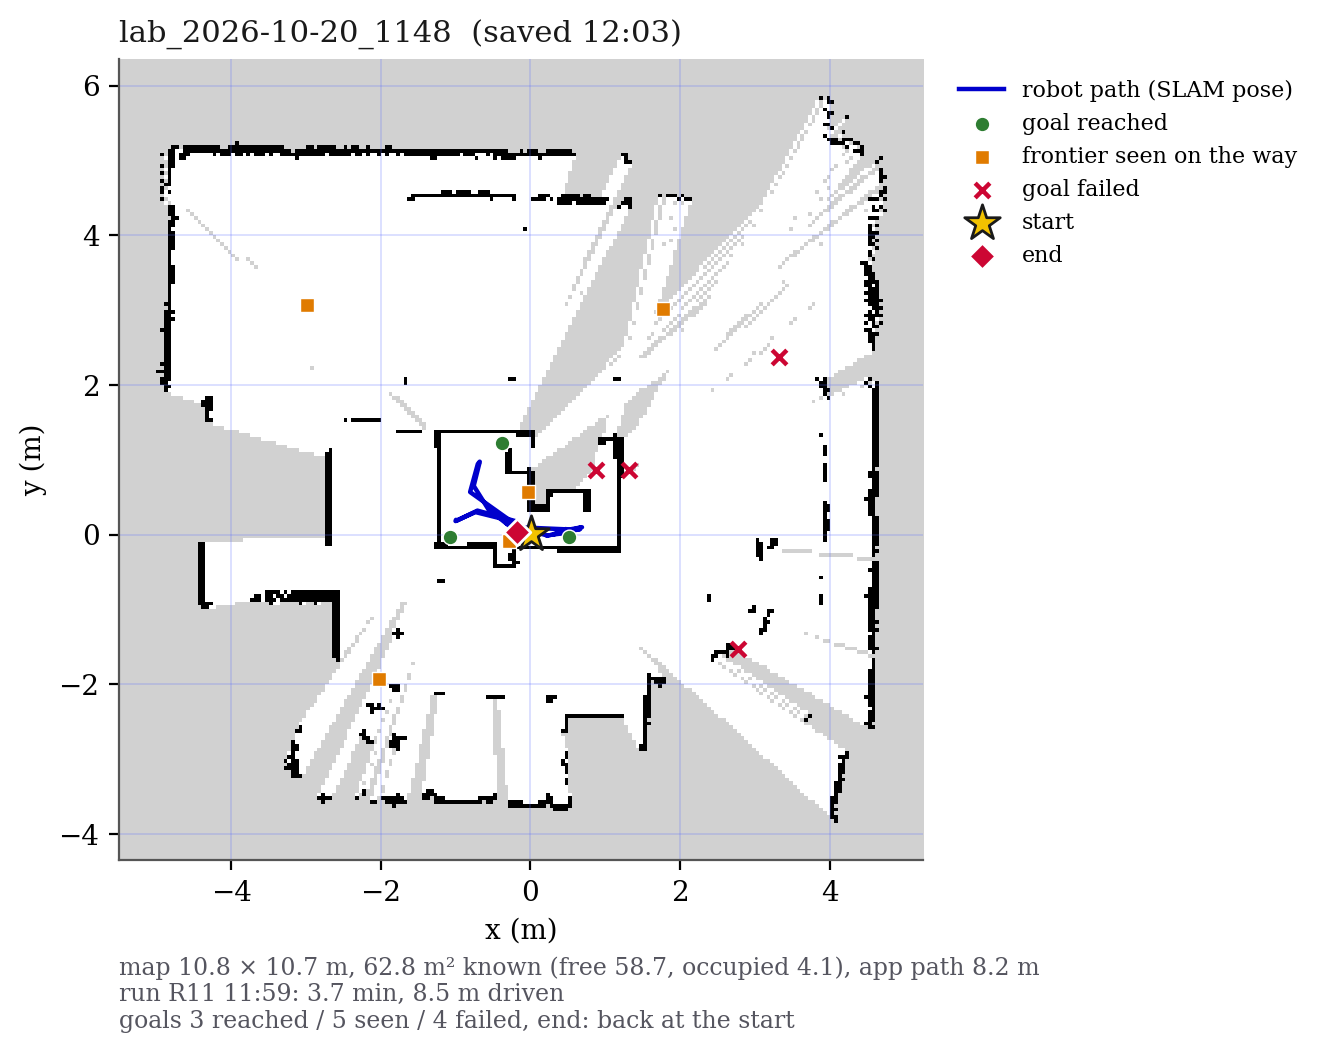
\includegraphics[width=\linewidth]{lab_2026-10-20_1148}\caption{R11}\end{subfigure}\hfill
\begin{subfigure}[t]{0.49\linewidth}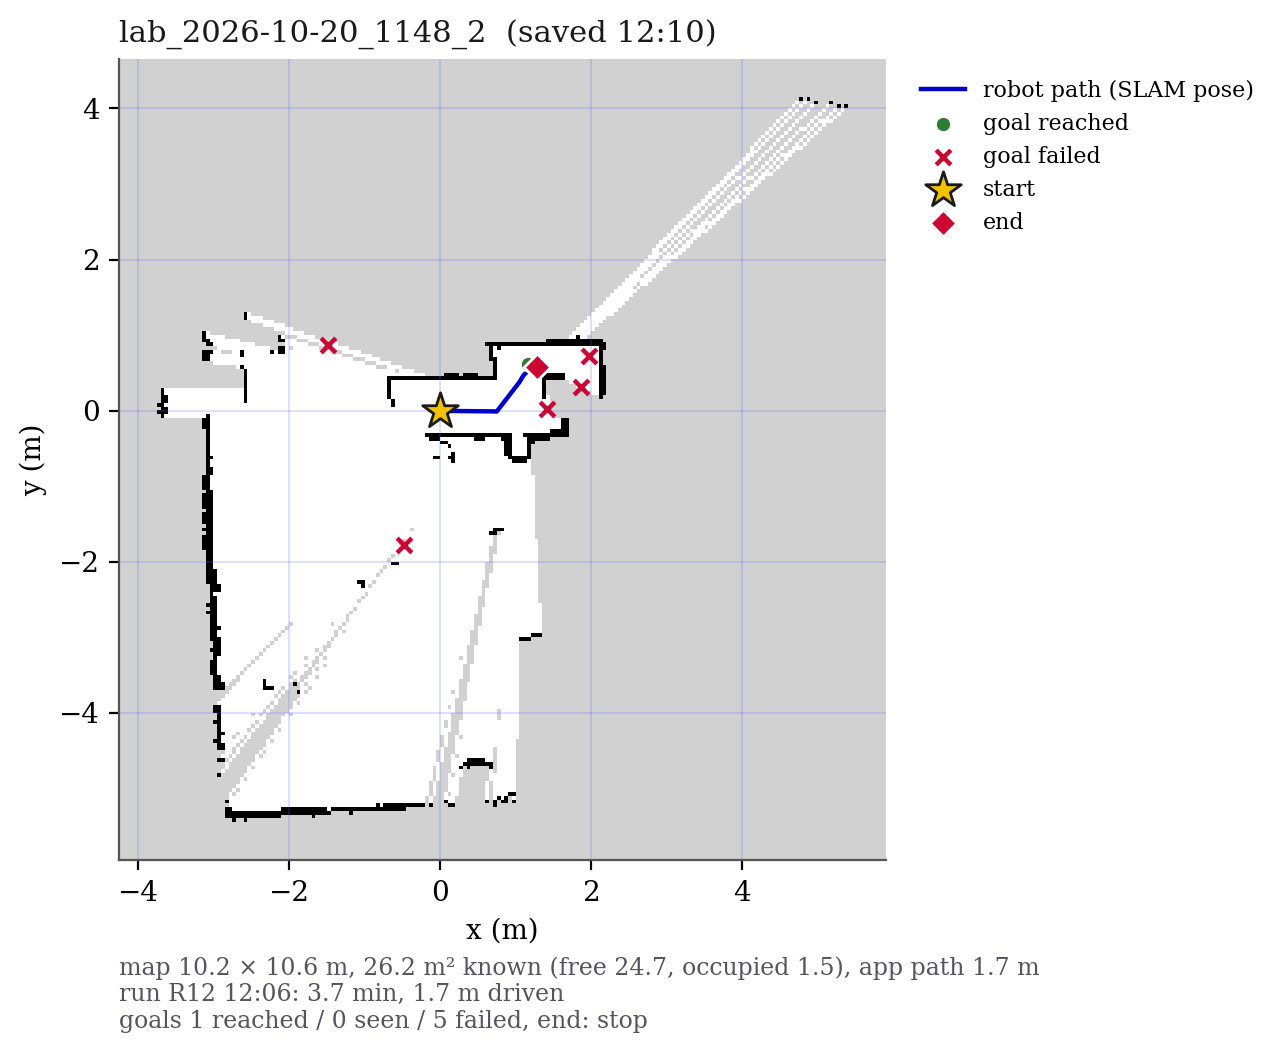
\includegraphics[width=\linewidth]{lab_2026-10-20_1148_2}\caption{R12}\end{subfigure}\\[4pt]
\begin{subfigure}[t]{0.49\linewidth}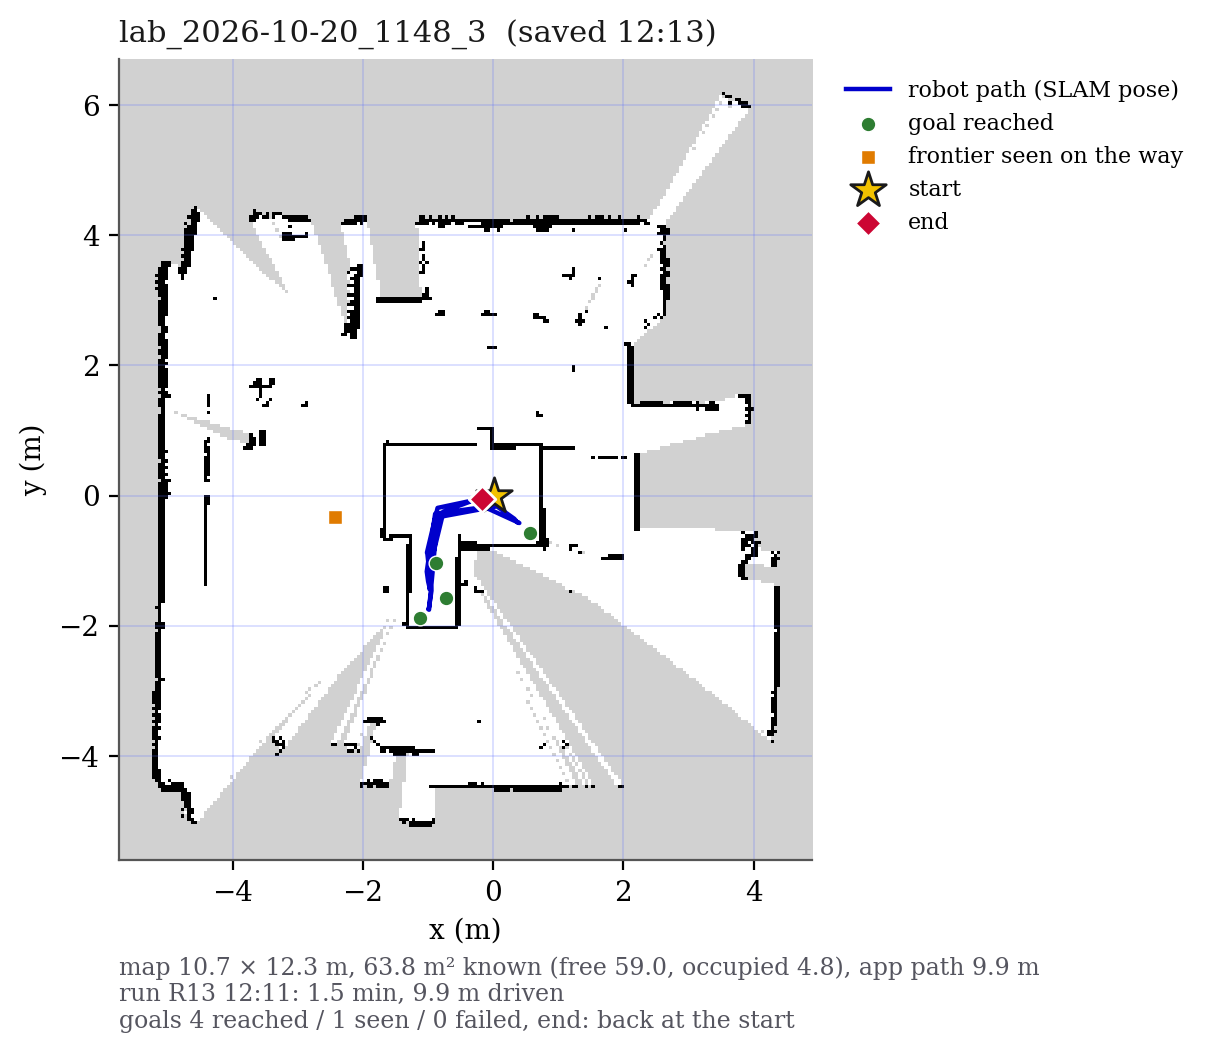
\includegraphics[width=\linewidth]{lab_2026-10-20_1148_3}\caption{R13}\end{subfigure}\hfill
\begin{subfigure}[t]{0.49\linewidth}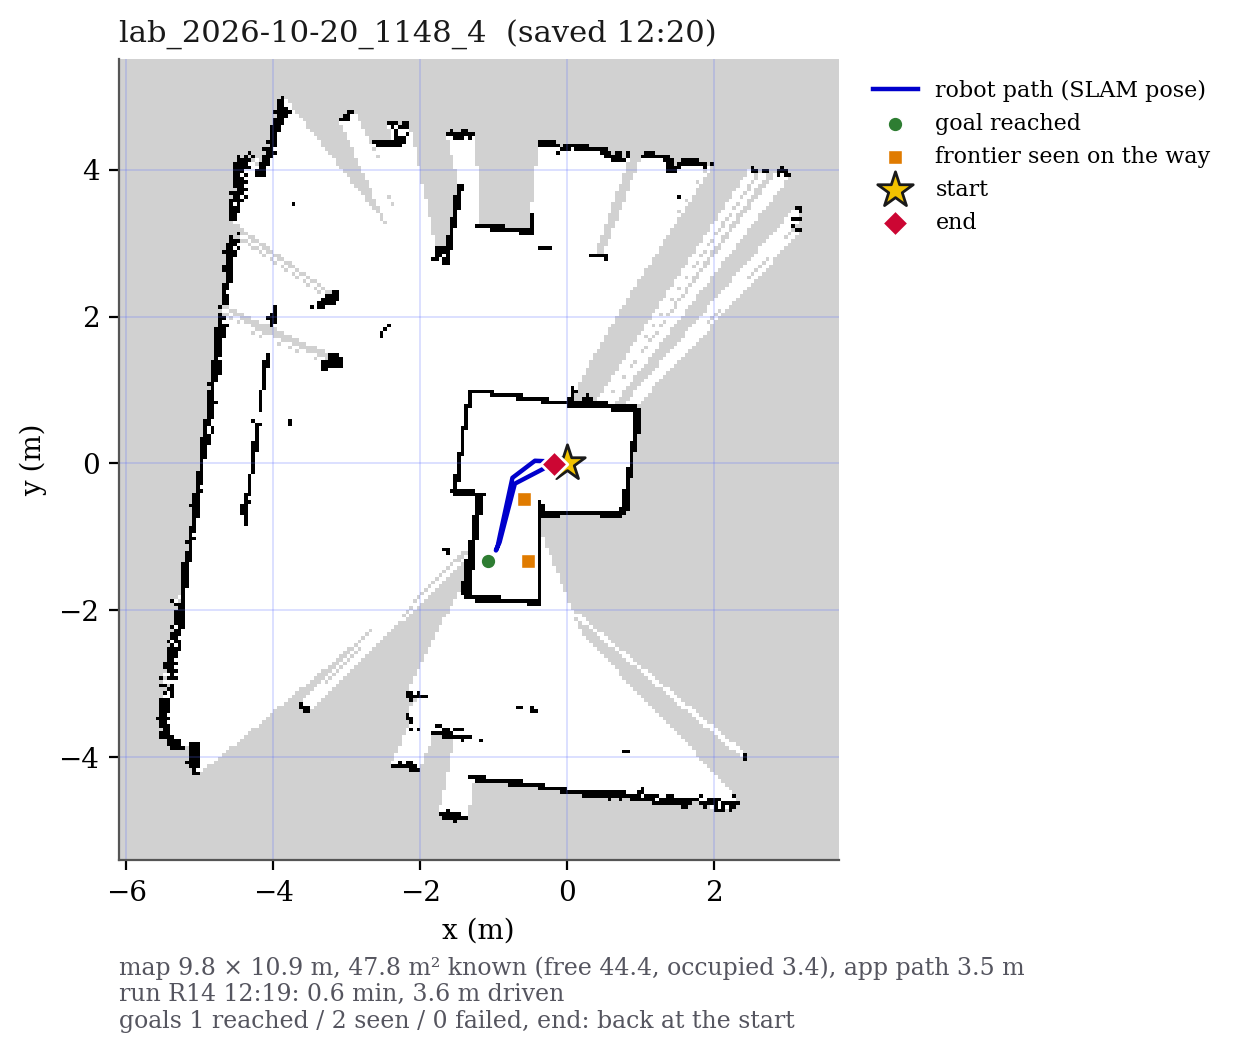
\includegraphics[width=\linewidth]{lab_2026-10-20_1148_4}\caption{R14}\end{subfigure}
\caption{Session D maps.}
\label{fig:mapsDE}
\end{figure}

\begin{figure}[H]
\centering
\begin{subfigure}[t]{0.49\linewidth}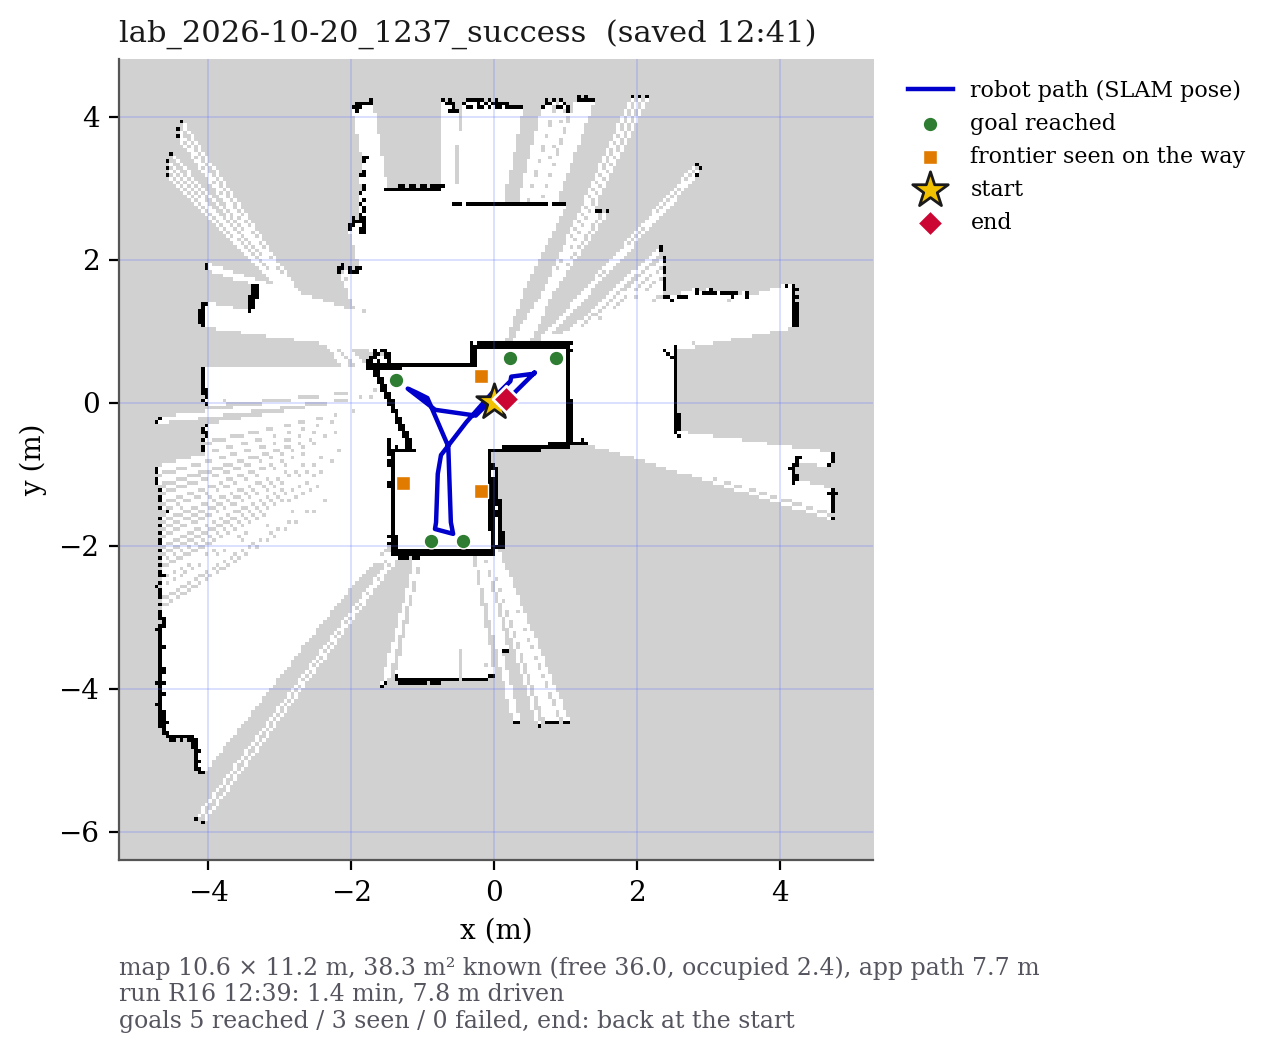
\includegraphics[width=\linewidth]{lab_2026-10-20_1237_success}\caption{R16}\end{subfigure}\hfill
\begin{subfigure}[t]{0.49\linewidth}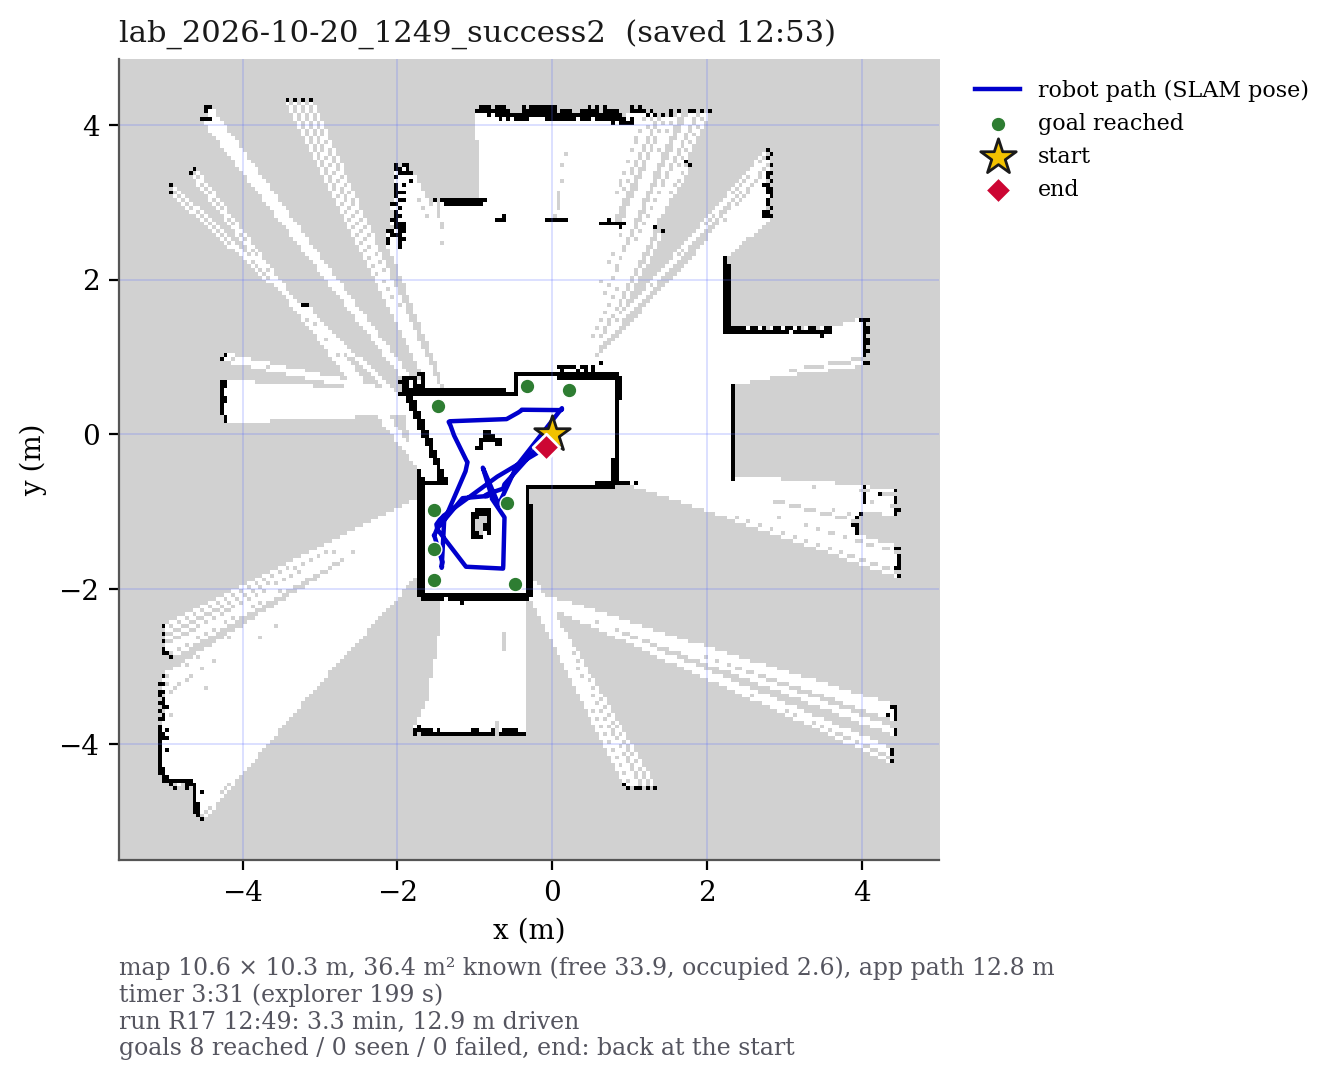
\includegraphics[width=\linewidth]{lab_2026-10-20_1249_success2}\caption{R17}\end{subfigure}\\[4pt]
\begin{subfigure}[t]{0.49\linewidth}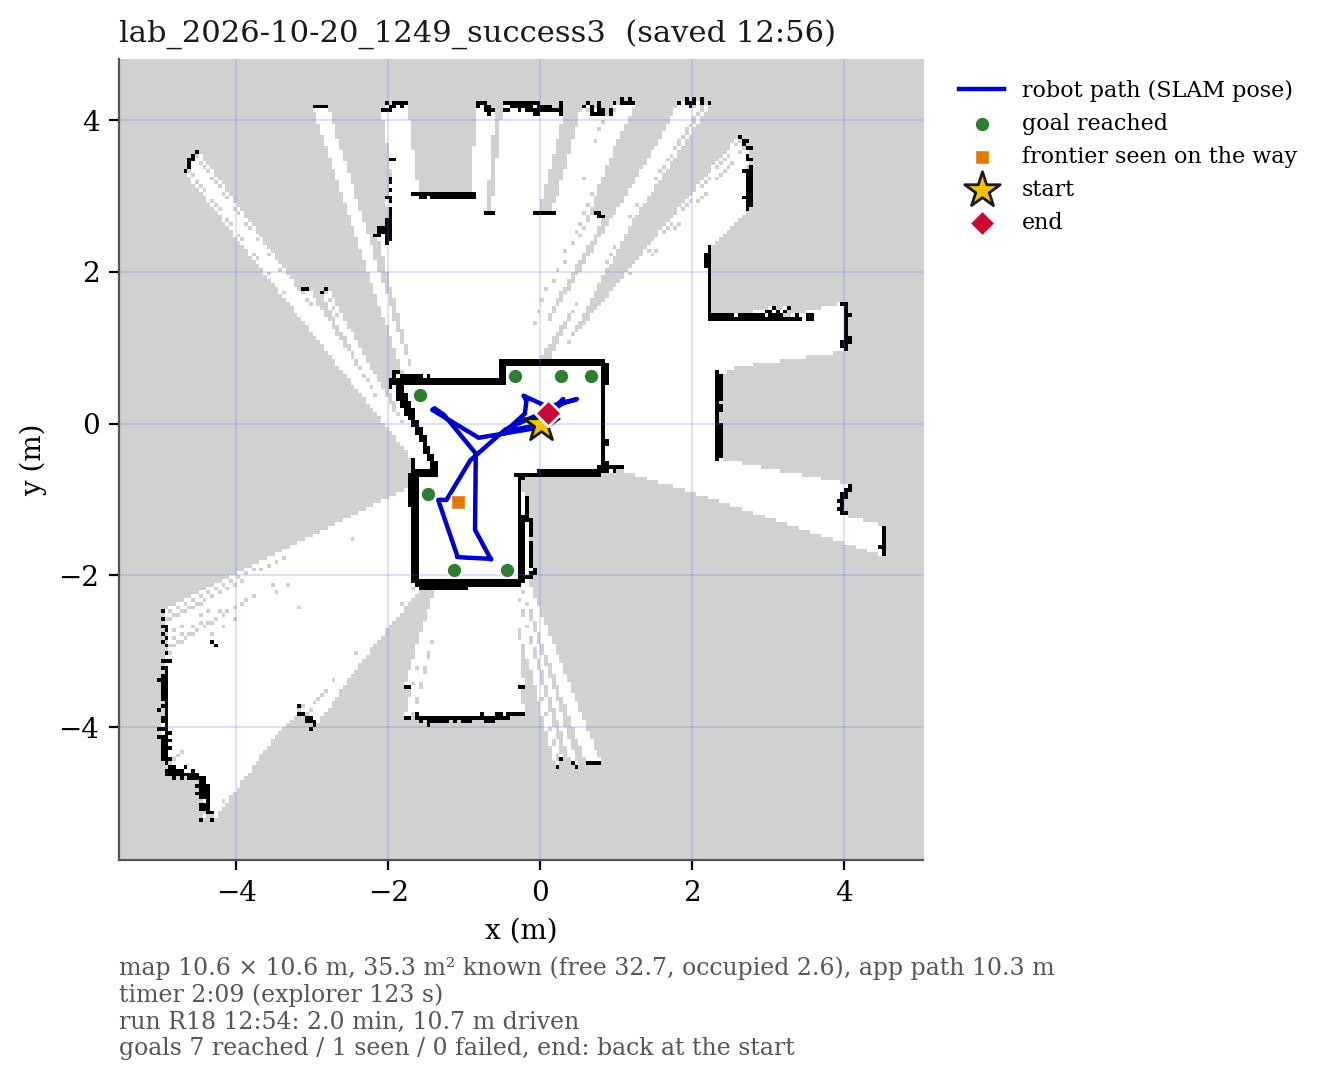
\includegraphics[width=\linewidth]{lab_2026-10-20_1249_success3}\caption{R18}\end{subfigure}
\caption{Session E maps.}
\end{figure}

\section{Findings and next steps}
\begin{enumerate}
\item \textbf{The full loop works in a bounded area.} In the enclosure, 7 of 9 runs explored to the
last frontier and drove home without help; the last six runs had no failed goal.
\item \textbf{Large open areas are not solved yet.} 82\,\% of goals aborted in session A and no run returned home.
Next: record Nav2's abort reason and the costmap at each failed goal, and test with a smaller inflation radius.
\item \textbf{Frontiers the robot cannot reach cost time.} Goals outside the enclosure (session D) failed one by one.
Next: drop frontiers that have no path in the global costmap before sending them.
\item \textbf{The battery rule trips on voltage dips.} Next: filter the voltage (for example a 5\,s mean)
before comparing it with 7.0\,V, and log the minimum voltage.
\item \textbf{Timing.} Use the explorer's elapsed time for the time to map an area; the app timer
now stores the session time with each map.
\end{enumerate}

\paragraph{Reproduce.} \texttt{python3 scripts/analyze\_day.py \&\& python3 scripts/make\_tables.py}, then
\texttt{pdflatex} this file twice in \texttt{report/}.

\end{document}
